\section{Software Structure}

\subsection{Joystick Control}

We use ROS write a node to switch between autonomous motor command and user control motor command.

\subsection{Waipoint Navigation}

We use GPS and IMU data to create Odometry. And it is filtered by a kalman filter then we pass our odometry to the navigation node to creat the motor command.

\subsection{Track and Trail}

To track the object on the water surface. We use pi-camera to get the image ahead of the boat. Then pass this image to object detection node. Once detect the object. we pass the bounding box of the object to the tracking node. Finally create a motor command to the Joystick node.

\begin{figure}[h]
	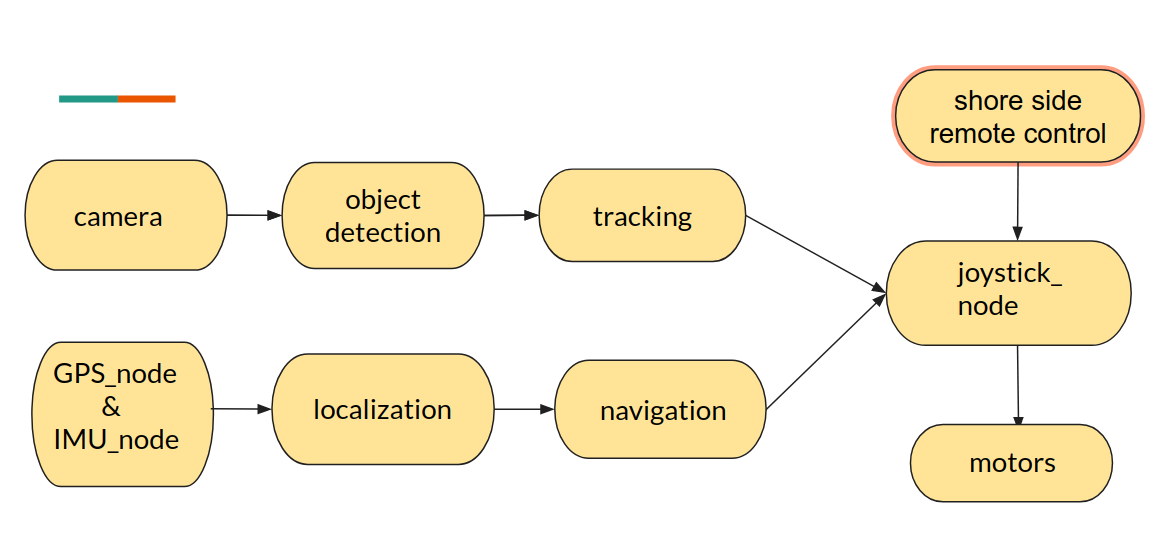
\includegraphics[width=0.8\columnwidth]{images/software_structure.png}
	\centering
	\caption{software structure}
	\label{figure:software_structure}
\end{figure}